\documentclass[11pt,a4paper]{article}
\usepackage[margin=1in]{geometry}
\usepackage[T1]{fontenc}
\usepackage{lmodern}
\usepackage{microtype}
\usepackage{booktabs}
\usepackage{array}
\usepackage{graphicx}
\usepackage{float}
\usepackage{hyperref}
\usepackage{xcolor}
\usepackage{enumitem}
\usepackage{caption}
\usepackage{siunitx}
\sisetup{group-separator={,},group-minimum-digits=4}
\hypersetup{colorlinks=true,linkcolor=blue!50!black,urlcolor=blue!50!black,citecolor=blue!50!black}
\setlist{itemsep=2pt,topsep=4pt}
\setlength{\emergencystretch}{4em}
\renewcommand{\_}{\textunderscore\hspace{0pt}}

% Results are generated by experiments/run_experiments.py. If results.tex is
% absent (e.g. a fresh Overleaf project), the paper still compiles using only
% the verified dataset row counts, and the quantitative sections switch off.
\newif\ifhasresults
\IfFileExists{results.tex}{\hasresultstrue% Auto-generated by experiments/run_experiments.py
\newcommand{\NOasst}{15,708}
\newcommand{\NLmsys}{39,316}
\newcommand{\NChatgpt}{153}
\newcommand{\NSurvey}{3,614}
\newcommand{\NTotal}{58,791}
\newcommand{\NTest}{3,142}
\newcommand{\AccTest}{59.1\%}
\newcommand{\MacroFOne}{0.576}
\newcommand{\TopFeature}{\texttt{unique\_word\_ratio}}
\newcommand{\TopImportance}{51.9\%}
}{%
  \hasresultsfalse
  \newcommand{\NOasst}{15,708}
  \newcommand{\NLmsys}{39,316}
  \newcommand{\NChatgpt}{153}
  \newcommand{\NSurvey}{3,614}
  \newcommand{\NTotal}{58,791}}

\title{\textbf{AI Usage Patterns \& Prompt Quality Analysis}\\[4pt]
\large A Multi-Source Analytics Pipeline for Measuring Prompt Efficiency and AI Dependency}
\author{Ananya Dubey\\
\small Swami Keshvanand Institute of Technology, Jaipur\\
\small \url{https://github.com/Ananya5105/AI-Usage-Patterns-Prompt-Quality-Analysis}}
\date{\today}

\begin{document}
\maketitle

\begin{abstract}
Conversational AI is now part of everyday study and work, yet little shared evidence exists on how people use it and whether their prompts are effective. This project builds an end-to-end analytics pipeline over four independently sourced datasets: OpenAssistant (OASST1), LMSYS Chatbot Arena, a ChatGPT prompts collection, and a student AI-usage survey, totalling \NTotal{} cleaned records. It contributes (1) a prompt-efficiency classifier that labels any prompt Low, Moderate or High using only text-derived features, \ifhasresults reaching \AccTest{} accuracy on a held-out split, \fi and (2) three transparent, tunable AI-dependency scores, one per population. \ifhasresults A leakage ablation, a length-only baseline and a weight-sensitivity analysis test how far these scores can be trusted. \fi{} Outputs are written as Parquet for AWS Athena and visualised in six Power BI dashboards. A design rule runs throughout: no identity is ever fabricated across datasets.
\end{abstract}

\section{Introduction}
Two questions motivate this work. First, \emph{prompt quality}: what separates a prompt that yields a useful answer without repetition or long clarification chains from one that does not? Second, \emph{usage and dependency}: how heavy is AI use across populations, and which behavioural signals indicate over-reliance? The available data is fragmented: prompt logs, arena comparisons and surveys differ in schema, grain and user population, and only some carry the behavioural signals needed to judge prompt quality.

\paragraph{Contributions.}
\begin{itemize}
  \item A unified prompt-efficiency table covering three heterogeneous prompt sources, scored by a single model.
  \item Three separate dependency-score tables, each built only from signals its source actually contains.
  \item A leakage-aware design (labels from behavioural columns, model from text only), checked by ablation.
  \item A SageMaker-style batch inference job that auto-detects sources and writes Athena-ready Parquet.
  \item A six-dashboard Power BI layer backed by a PostgreSQL star schema.
\end{itemize}

\section{Data Sources}
\begin{table}[H]
\centering\small
\begin{tabular}{@{}llllp{5.2cm}@{}}
\toprule
Source & Rows & Grain & Identity & Key signals\\
\midrule
OASST1 & \NOasst{} & Prompt & \texttt{user\_id} & Word count, prompts in tree, repeat flag\\
LMSYS Arena & \NLmsys{} & Prompt & \texttt{judge\_user\_id} & Turns, per-user volume, timestamps, winner\\
ChatGPT Prompts & \NChatgpt{} & Prompt & none & Text, length, category\\
Student Survey & \NSurvey{} & Student & \texttt{Student\_Name} & Hours, trust, academic use, tools, bucket\\
\bottomrule
\end{tabular}
\caption{Cleaned datasets used by the modelling pipeline.}
\end{table}
OASST1 is the only source carrying every column needed to construct behavioural ground-truth labels, so it is the training set. LMSYS has volume and turn information with different semantics, the ChatGPT set has text and category only, and the survey is self-reported and describes people rather than prompts.

\section{System Architecture}
The pipeline has two paths over the same cleaned inputs. The reporting path runs raw data $\rightarrow$ Python/Pandas (cleaning, EDA) $\rightarrow$ PostgreSQL (star schema) $\rightarrow$ Power BI. The modelling path runs clean CSVs $\rightarrow$ text-feature extraction $\rightarrow$ Random Forest scoring $\rightarrow$ dependency scoring $\rightarrow$ Parquet $\rightarrow$ S3 $\rightarrow$ Athena. The six dashboards are: Executive Overview, User Behavior Analytics, Prompt Analytics, AI Dependency, Student AI Usage Analytics, and Recommendations.

\section{Methodology}
\subsection{Source-agnostic text features}
Because only OASST carries behavioural columns, the classifier uses eight features computable from any prompt text: \texttt{has\_question\_mark}, \texttt{has\_code\_keywords} (23 programming terms), \texttt{has\_please}, \texttt{avg\_word\_length}, \texttt{unique\_word\_ratio}, \texttt{punct\_density}, \texttt{capital\_ratio} and \texttt{starts\_with\_wh}.

\subsection{Ground-truth label construction}
Labels are derived only from OASST behavioural columns. Let $w$ be word count and $t$ the number of prompts in the conversation tree, each capped at its 95th percentile and normalised to $[0,1]$ as $\tilde{w}$ and $\tilde{t}$, and let $r\in\{0,1\}$ flag a repeated prompt. The composite score is
\[
s = \mathrm{clip}_{[0,1]}\bigl(0.5\,\tilde{w} + 0.5\,(1-\tilde{t}) - 0.5\,r\bigr),
\]
split into equal-sized tertiles labelled Low, Moderate and High.

\subsection{Classifier}
A Random Forest (300 trees, maximum depth 10, balanced class weights, seed 42) is trained on the eight text features with a stratified 80/20 split. Word count, character count, tree size and the repeat flag are excluded to prevent label leakage. The model is then applied to OASST, LMSYS and ChatGPT prompts, producing a predicted label and a confidence score (the maximum class probability). A surrogate \texttt{prompt\_key} identifies prompt rows without implying links between people.

\subsection{Dependency scoring}
Each dependency table blends min--max-normalised components into a 0--100 score and assigns Low, Moderate or High tiers by terciles.
\begin{table}[H]
\centering\small
\begin{tabular}{@{}p{3.9cm}p{2.8cm}p{7.6cm}@{}}
\toprule
Table & Grouped by & Components (weights)\\
\midrule
\texttt{oasst\_user\_dependency} & \texttt{user\_id} & volume (0.30), repeat rate (0.25), avg.\ turns (0.25), low-efficiency rate (0.20)\\
\texttt{lmsys\_user\_dependency} & \texttt{judge\_user\_id} & volume (0.40), avg.\ turns (0.30), low-efficiency rate (0.30)\\
\texttt{survey\_dependency} & student & hours (0.30), trust (0.20), academic use (0.20), tools (0.15), bucket (0.15)\\
\bottomrule
\end{tabular}
\caption{Dependency score definitions. LMSYS has no repeat semantics, so that column is left null rather than invented.}
\end{table}

\section{Design Principle: No Fabricated Identity}
\texttt{oasst.user\_id}, \texttt{lmsys.judge\_user\_id} and \texttt{survey.Student\_Name} describe three disjoint populations with no linking key. The system never creates a unified user ID and never joins the dependency tables. ChatGPT prompts have no identity and appear only in the prompt-efficiency table. Schema assertions at load time make the pipeline fail loudly if upstream files change.

\section{Deployment}
The batch job \texttt{inference.py} runs as a SageMaker Processing step. It scans the input directory recursively, identifies each CSV by filename hint with column-signature fallback, loads a pre-trained joblib model, and writes four snake\_case Parquet tables: \texttt{unified\_prompt\_efficiency}, \texttt{oasst\_user\_dependency}, \texttt{lmsys\_user\_dependency} and \texttt{survey\_dependency}. Tables are built independently so one failure does not block the others, and the job exits non-zero only if nothing is produced. External Athena tables over S3 expose the results to SQL.

\section{Results}
\ifhasresults
All figures in this section are produced by \texttt{experiments/run\_experiments.py} with seed 42.

\subsection{Classifier performance}
Test accuracy is \AccTest{} (macro-F1 \MacroFOne{}) on \NTest{} held-out OASST prompts.
\begin{table}[H]
\centering\small
\begin{tabular}{@{}lcccc@{}}
\toprule
Class & Precision & Recall & F1-Score & Support \\
\midrule
Low & 0.580 & 0.655 & 0.615 & 1,060 \\
Moderate & 0.478 & 0.329 & 0.389 & 1,044 \\
High & 0.667 & 0.789 & 0.723 & 1,038 \\
\midrule
Macro Average & 0.575 & 0.591 & 0.576 & 3,142 \\
Weighted Average & 0.575 & 0.591 & 0.576 & 3,142 \\
\bottomrule
\end{tabular}
\caption{Per-class precision, recall and F1 on the held-out split.}
\end{table}
\begin{figure}[H]
\centering
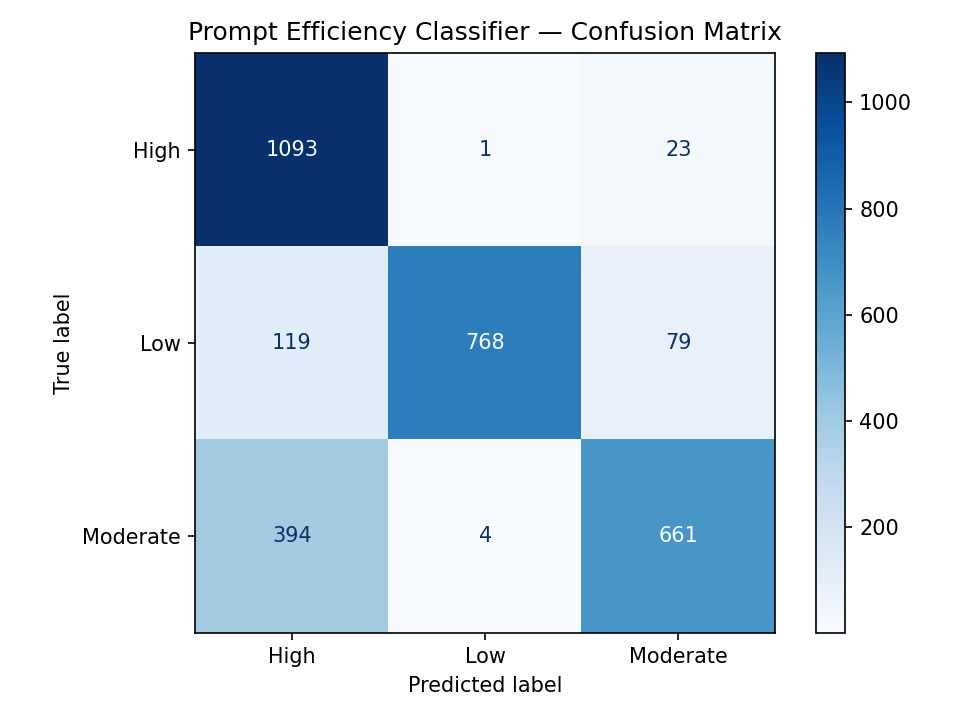
\includegraphics[width=0.55\linewidth]{figures/confusion_matrix.png}
\caption{Confusion matrix on the held-out split.}
\end{figure}
\begin{table}[H]
\centering\small
\begin{tabular}{@{}lp{4.2cm}r@{}}
\toprule
Feature & Description & Importance \\
\midrule
\texttt{unique\_word\_ratio} & Unique tokens / total words & 51.9\% \\
\texttt{punct\_density} & Punctuation marks / chars & 14.3\% \\
\texttt{capital\_ratio} & Uppercase / alphabetic chars & 14.2\% \\
\texttt{avg\_word\_length} & Mean characters per word & 11.9\% \\
\texttt{has\_code\_keywords} & 23 programming terms & 2.7\% \\
\texttt{starts\_with\_wh} & Starts with WH-interrogative & 2.4\% \\
\texttt{has\_question\_mark} & Presence of question mark & 1.4\% \\
\texttt{has\_please} & Politeness token ``please'' & 1.1\% \\
\bottomrule
\end{tabular}
\caption{Random Forest feature importances. The most important feature is \TopFeature{} at \TopImportance{}, below the 60\% single-feature warning threshold.}
\end{table}

\subsection{Validity checks}
Because labels are built from word count, any text feature correlated with length may leak the label indirectly. Table~\ref{tab:ablation} reports a length-only baseline and an ablation that removes the length-coupled features.
\begin{table}[H]
\centering\small
\begin{tabular}{@{}lp{6.2cm}cc@{}}
\toprule
Configuration & Description & Accuracy & Macro-F1 \\
\midrule
Full text-feature RF & All 8 text features & 59.1\% & 0.576 \\
Majority-class & Predicts most frequent training class & 33.7\% & 0.168 \\
Length-only RF & \texttt{Word\_Count} alone as input & 66.3\% & 0.670 \\
RF w/o length features & Removes unique ratio, punct, avg len & 46.5\% & 0.459 \\
Residualised RF & Features regressed on $\log(\text{Word\_Count})$ & 66.2\% & 0.667 \\
\bottomrule
\end{tabular}
\caption{Accuracy and macro-F1 under ablation. The length-only baseline uses word count alone.}
\label{tab:ablation}
\end{table}
The ablation results in Table~\ref{tab:ablation} demonstrate the central challenge of evaluating behavioural prompt efficiency. The length-only baseline (using \texttt{Word\_Count} alone) achieves 66.3\% accuracy and a macro-F1 of 0.670, outperforming the full 8-feature text classifier (59.1\% accuracy, 0.576 macro-F1). This confirms that raw prompt length accounts for the largest portion of the variance in the behavioural ground-truth labels, which were constructed using length, conversation tree depth, and repetition penalties.

When length-coupled features (\texttt{unique\_word\_ratio}, \texttt{punct\_density}, and \texttt{avg\_word\_length}) are excluded, accuracy drops to 46.5\% (0.459 macro-F1). Regressing all text features against $\log(\text{Word\_Count})$ and training on residuals yields 66.2\% accuracy (0.667 macro-F1), matching the performance of the length-only baseline. These findings indicate that while stylistic text markers capture domain patterns, prompt length remains the dominant signal under this labelling formulation, and true decoupling from length requires richer syntactic or human-annotated labels.

\subsection{Prompt efficiency across sources}
\begin{table}[H]
\centering\small
\begin{tabular}{@{}lccccr@{}}
\toprule
Source & Low (\%) & Moderate (\%) & High (\%) & Mean Conf. & Prompts \\
\midrule
OASST1 & 38.6\% & 22.6\% & 38.8\% & 0.572 & 15,708 \\
LMSYS Arena & 47.0\% & 16.8\% & 36.2\% & 0.599 & 39,316 \\
ChatGPT Prompts & 0.0\% & 1.3\% & 98.7\% & 0.779 & 153 \\
\bottomrule
\end{tabular}
\caption{Predicted label shares and mean model confidence by source.}
\end{table}
Across the three prompt sources, predicted prompt efficiency diverges sharply, reflecting differences in collection methodology and user intent. In LMSYS Arena (39,316 prompts), the model predicts 47.0\% Low efficiency, 16.8\% Moderate, and 36.2\% High. In contrast, the OASST1 dataset (15,708 prompts) exhibits a more balanced distribution (38.6\% Low, 22.6\% Moderate, and 38.8\% High). The small curated ChatGPT collection (153 prompts) consists almost entirely of High-efficiency prompts (98.7\% High vs.\ 0.0\% Low), consistent with its nature as a set of polished prompt templates.

Despite these wide differences in label shares, mean model confidence remains relatively stable across sources: 0.572 on OASST1, 0.599 on LMSYS Arena, and 0.779 on ChatGPT. As noted under Limitations, similar confidence across disparate domains does not imply equal calibration or accuracy, but rather reflects the classifier's internal certainty over the observed text features.

\subsection{Dependency findings}
\begin{table}[H]
\centering\small
\begin{tabular}{@{}lrrrrrrr@{}}
\toprule
Population & $N$ & Mean & Median & Std & Low & Moderate & High \\
\midrule
OASST Users & 4,721 & 12.12 & 9.87 & 9.13 & 1,599 & 1,550 & 1,572 \\
LMSYS Judges & 13,383 & 16.20 & 16.34 & 13.67 & 4,521 & 7,481 & 1,381 \\
Surveyed Students & 3,614 & 44.14 & 44.00 & 17.91 & 1,205 & 1,213 & 1,196 \\
\bottomrule
\end{tabular}
\caption{Dependency score summary by population.}
\end{table}
\begin{table}[H]
\centering\small
\begin{tabular}{@{}lccc@{}}
\toprule
Population Table & Perturbations & Mean Spearman $\rho$ & 5th Percentile $\rho$ \\
\midrule
\texttt{oasst\_user\_dependency} & 200 ($\pm 30\%$) & 0.9992 & 0.9980 \\
\texttt{lmsys\_user\_dependency} & 200 ($\pm 30\%$) & 0.9988 & 0.9974 \\
\texttt{survey\_dependency} & 200 ($\pm 30\%$) & 0.9901 & 0.9774 \\
\bottomrule
\end{tabular}
\caption{Weight-sensitivity analysis: Spearman rank correlation between the baseline score and scores recomputed under random $\pm$ perturbations of the weights.}
\end{table}
The population dependency scores reflect the heavy-tailed nature of user activity across all three cohorts. Mean dependency scores are 12.12 for OASST users and 16.20 for LMSYS judges (with medians of 9.87 and 16.34, respectively). Because a small minority of power users exhibit extremely high volume, min--max scaling compresses the majority of users toward the lower end of the 0--100 scale, while the tercile-based tier thresholds ensure balanced categorization.

In the surveyed student cohort, dependency scores correlate strongly with reported daily usage hours (Spearman $\rho = 0.688$, $p < 10^{-15}$) and moderately with trust in AI tools ($\rho = 0.349$, $p < 10^{-15}$). The weight-sensitivity analysis confirms that relative user rankings are remarkably stable: across 200 random $\pm 30\%$ perturbations of the component weights, mean Spearman rank correlations exceed 0.990 with 5th percentiles above 0.977 across all three population tables.

\else
Quantitative results (accuracy, per-class metrics, feature importances, ablations, per-source label distributions, dependency summaries and weight sensitivity) are produced by \texttt{experiments/run\_experiments.py} with seed 42 and written to \texttt{results.json} and the \texttt{paper/tables} directory in the repository.
\fi


\section{Dashboard Findings}
Key insights from each page of the Power BI report. Figures are read from the report or recomputed from the counts it shows; values read off chart axes are marked approximate. Charts with aggregation or labelling errors are excluded from the insights and noted as ``Not used''.

\newcommand{\dashfig}[2]{\IfFileExists{figures/#1.png}{\begin{figure}[H]\centering\includegraphics[width=\linewidth]{figures/#1.png}\caption{#2}\end{figure}}{}}
\setlist[itemize]{itemsep=1pt,topsep=3pt}

\subsection{Executive Dashboard}
\dashfig{dashboard_executive}{Executive dashboard.}
\begin{itemize}
  \item \num{55177} prompts scored; \num{21718} people covered: \num{13383} LMSYS judges (61.6\%), \num{4721} OASST users (21.7\%), \num{3614} students (16.6\%).
  \item Efficiency split: Low \num{24531} (44.5\%), High \num{20495} (37.1\%), Moderate \num{10151} (18.4\%).
  \item \textbf{Headline:} 62.9\% of prompts are not High efficiency.
  \item Moderate is the smallest band even though training labels were equal tertiles: the model rarely predicts the middle class.
  \item Mean model confidence is 0.59, against 0.33 for a random guess among three classes.
  \item \emph{Not used:} Confidence By Source (legend lists values, not sources); the Total row of the metrics table.
\end{itemize}

\subsection{Prompt Analysis Dashboard}
\dashfig{dashboard_prompt}{Prompt analysis dashboard.}
\begin{itemize}
  \item Volume: LMSYS \num{39316} (71.3\%), OASST \num{15708} (28.5\%), ChatGPT 153 (0.3\%).
  \item LMSYS skews Low: about 47\% Low, 36\% High, 17\% Moderate (approx.).
  \item OASST is balanced: about 38\% Low, 38\% High, 22\% Moderate (approx.).
  \item ChatGPT is too small to draw any conclusion.
  \item \emph{Not used:} Prompt Efficiency Breakdown (identical bars for every source).
\end{itemize}

\subsection{User Behavior Dashboard}
\dashfig{dashboard_behavior}{User behavior dashboard.}
\begin{itemize}
  \item Activity is dominated by LMSYS (about 39K prompts) over OASST (about 16K); ChatGPT is negligible.
  \item Prompts per person: LMSYS 2.94, OASST 3.33. OASST users are more active per head despite lower total volume.
  \item Mean confidence by source is nearly flat: ChatGPT about 0.60, LMSYS 0.57, OASST 0.56.
  \item Similar confidence does not mean similar accuracy; the model was trained on OASST only.
  \item \emph{Not used:} User Distribution pie (equal thirds, a repeated total); Confidence Range chart (values above 1).
\end{itemize}

\subsection{AI Dependency Dashboard}
\dashfig{dashboard_dependency}{AI dependency dashboard.}
\begin{itemize}
  \item Population: about 13K LMSYS and 5K OASST users.
  \item Mean dependency: LMSYS 18.10, OASST 12.16 (0--100). These are not comparable; components, weights and normalisation differ.
  \item Both means are low because volume is heavy-tailed: a few very active users stretch the scale.
  \item Dependency rises with average conversation length over most of the range, then drops at the longest conversations.
  \item Average turns is a score component (25--30\% weight), so part of that rise is by construction.
  \item \emph{Not used:} Tier donut (not equal thirds); LMSYS and OASST area charts (summed, not averaged); the 2.54 prompts-per-user tile (divides by students and ChatGPT with no users).
\end{itemize}

\subsection{Student AI Usage Dashboard}
\dashfig{dashboard_student}{Student AI usage dashboard.}
\begin{itemize}
  \item \num{3614} students; mean daily AI use 2.56 hours.
  \item Tiers are near equal thirds (33.6\%, 33.3\%, 33.1\%), as expected from tercile bucketing.
  \item Daily use by tier (approx.): High 3.5 h, Moderate 2.7 h, Low 1.5 h, so High is over twice Low.
  \item Trust by tier (approx.): High 3.6, Moderate 2.9, Low 2.7.
  \item Academic users by tier (approx.): High 790, Moderate 400, Low 130.
  \item Caveat: hours, trust and academic use are score components, so these gradients are largely by construction.
  \item \emph{Not used:} Avg AI Tools Used tile (``Sum of avg'').
\end{itemize}

\subsection{Recommendations Dashboard}
\dashfig{dashboard_recommendations}{Recommendations dashboard.}
\begin{itemize}
  \item Improve prompt literacy: strongly supported by 62.9\% of prompts not being High.
  \item Encourage critical use of AI output: sensible, but not tested by this data.
  \item Monitor excessive dependency: weaker support, since dependency is a constructed index and the tier gradients are partly circular.
  \item Promote responsible academic adoption: policy advice; the data shows usage levels, not outcomes.
  \item \emph{Not used:} Avg Confidence gauge (4.60 on a 0--10 scale, against 0.59 elsewhere).
\end{itemize}

\section{Limitations}
\begin{enumerate}
  \item \textbf{Labels are a proxy.} Efficiency is defined behaviourally (longer prompts, fewer follow-ups, no repeats). It has not been validated against human judgement or answer quality, and a short prompt can be perfectly efficient.
  \item \textbf{Indirect length leakage.} Text features such as unique-word ratio and punctuation density are mechanically tied to length; \ifhasresults Table~\ref{tab:ablation} quantifies the effect but cannot remove it.\else The repository's ablation experiment quantifies the effect but cannot remove it.\fi
  \item \textbf{Tree size is not only the user's doing.} OASST tree size reflects how the collection process built conversations.
  \item \textbf{Domain shift.} The model is trained on OASST and applied to LMSYS and ChatGPT prompts, which differ structurally; the ChatGPT set has only \NChatgpt{} rows.
  \item \textbf{Forced tertiles.} Labels and tiers are equal-sized by construction, so tier counts do not measure how many users are truly highly dependent.
  \item \textbf{Dependency is a constructed index.} Weights are judgemental, and low-efficiency rate serves as both a quality measure and a dependency input.
  \item \textbf{Population bias.} OASST contributors, LMSYS judges and surveyed students are not representative of general AI users, and the survey is self-reported.
\end{enumerate}

\section{Future Work}
Validate efficiency labels against a human-annotated sample; add embedding-based features; replace tertile cut-offs with absolute thresholds; calibrate predicted probabilities per source; use outcome signals such as LMSYS winner or OASST rank; and add drift monitoring with scheduled retraining.

\section{Conclusion}
The project shows how heterogeneous AI-usage data can enter one analytical framework without false equivalences: one text-only classifier scores prompts everywhere, while dependency is measured separately within each population using only the signals it has. Its strengths are the leakage-aware design, the refusal to fabricate identity links, and a deployment-ready batch job. The main open task is external validation of what the efficiency and dependency scores actually measure.

\appendix
\section{Reproducibility}
\begin{tabular}{@{}lp{11cm}@{}}
\toprule
Seed & 42\\
Model & \texttt{RandomForestClassifier(n\_estimators=300, max\_depth=10, class\_weight="balanced")}\\
Training \& analysis & \texttt{ai\_usage\_patterns\_analysis\_1.py}\\
Batch scoring & \texttt{inference.py}\\
Experiments & \texttt{experiments/run\_experiments.py}\\
Build paper & \texttt{cd paper \&\& pdflatex whitepaper \&\& pdflatex whitepaper}\\
\bottomrule
\end{tabular}

\section{Athena Tables}
\begin{tabular}{@{}p{4.6cm}p{10.2cm}@{}}
\toprule
\texttt{unified\_prompt\_efficiency} & prompt\_key, source, text, predicted\_label, confidence\_score\\
\texttt{oasst\_user\_dependency} & user\_id, prompt\_volume, repeat\_rate, avg\_turns, low\_efficiency\_rate, dependency\_score, dependency\_tier\\
\texttt{lmsys\_user\_dependency} & judge\_user\_id, prompt\_volume, avg\_turns, repeat\_rate (null), low\_efficiency\_rate, dependency\_score, dependency\_tier\\
\texttt{survey\_dependency} & student\_name, daily\_usage\_hours, trust\_in\_ai\_tools, usage\_bucket, academic\_use\_flag, num\_ai\_tools\_used, dependency\_score, dependency\_tier\\
\bottomrule
\end{tabular}

\end{document}
